% ============================================================
% GNNocRoute: Topology-Aware Periodic Routing Optimization for NoC
% A Feasibility Study using Graph Neural Networks
%
% IEEEtran LaTeX
% Compile with: pdflatex → bibtex → pdflatex → pdflatex
% TeXshop: select "LaTeX" engine, run twice
% ============================================================
% Author: Le Tien Hieu, IEEE Member
% VNU-ITI, Vietnam National University, Hanoi
% Date: 14/05/2026
% ============================================================

\documentclass[conference]{IEEEtran}

% ---- Encoding & Fonts ----
\usepackage[utf8]{inputenc}
\usepackage[T1]{fontenc}

% ---- Math ----
\usepackage{amsmath,amssymb,amsfonts}

% ---- Graphics ----
\usepackage{graphicx}
\usepackage{epsfig}
\usepackage[justification=centering]{caption}

% ---- Tables ----
\usepackage{booktabs}
\usepackage{array}
\usepackage{multirow}

% ---- References ----
\usepackage{cite}
\usepackage{hyperref}

% ---- Misc ----
\usepackage{textcomp}
\usepackage{xcolor}

\hypersetup{
    colorlinks=true,
    linkcolor=blue,
    citecolor=blue,
    urlcolor=blue
}

% ---- Figure Path ----
\graphicspath{{./figures/}}

% ---- Document ----
\begin{document}

\title{GNNocRoute: Topology-Aware Periodic Routing Optimization for Network-on-Chip}

\author{
    \IEEEauthorblockN{Le Tien Hieu\textsuperscript{1}, \textit{IEEE Member}}
    \IEEEauthorblockA{\textsuperscript{1}VNU-ITI, Vietnam National University, Hanoi\\
    Email: hieult@vnu.edu.vn}
}

\maketitle

\begin{abstract}
Network-on-Chip (NoC) is the communication backbone for modern multi-core System-on-Chips. Conventional deterministic routing algorithms such as XY dimension-order routing suffer from congestion imbalance---our graph-theoretic analysis across seven topologies shows that an $8\times8$ mesh under XY routing achieves a congestion imbalance of 0.475, with central nodes exhibiting $2-3\times$ higher betweenness centrality than edge nodes.

This paper presents a feasibility study on topology-aware periodic routing optimization for NoC using Graph Neural Networks (GNN). We report four preliminary experimental findings. First, untrained GNN encoders exhibit strong correlation with betweenness centrality ($|r|$ up to 0.978 on Mesh $4\times4$), suggesting that topology-aware representations emerge implicitly. Second, cross-topology generalization experiments indicate that relative node importance rankings transfer across mesh sizes (Pearson $r \approx 0.96$), though absolute scaling remains topology-specific. Third, measured inference latency on CPU of approximately $10^6$ cycles per forward pass on an $8\times8$ mesh confirms that per-packet GNN inference is impractical under NoC timing constraints, motivating periodic policy optimization as a necessary design alternative. Fourth, GNN inference time scales approximately $O(N)$ with the number of nodes.

These findings provide initial evidence that topology-aware representations can be extracted via GNN encoding, and that periodic routing optimization offers a feasible path toward topology-generalizable adaptive routing on NoC. We discuss implications and limitations of this early-stage investigation.
\end{abstract}

\begin{IEEEkeywords}
Network-on-Chip, Graph Neural Networks, Periodic Routing Optimization, Feasibility Study, Congestion Analysis
\end{IEEEkeywords}

% ════════════════════════════════════════════════
\section{Introduction}
\label{sec:intro}
% ════════════════════════════════════════════════

Network-on-Chip (NoC) has become the standard communication infrastructure for modern multi-core System-on-Chips (SoCs) and AI accelerators such as Google TPU and NVIDIA Grace Hopper~\cite{mirhoseini2021}. In NoC, routers connect via links forming a graph structure. The routing algorithm determines packet paths and directly affects system performance.

XY Dimension-Order Routing is widely used in commercial NoCs~\cite{wang2022maar} due to its simplicity. However, XY routing always selects the same path for each (source, destination) pair regardless of congestion. Our graph analysis on seven topologies reveals:

\begin{itemize}
    \item An $8\times8$ mesh with XY routing achieves a \textbf{congestion imbalance} of \textbf{0.475}---nearly half of all links experience uneven load distribution.
    \item Central nodes in a $4\times4$ mesh exhibit Betweenness Centrality (BC) $\approx 0.25$, which is $2-3\times$ higher than edge nodes.
    \item A k=4 Fat-Tree has aggregation switches with BC up to \textbf{0.42}---all inter-pod traffic must pass through these two switches.
\end{itemize}

These results demonstrate that \textbf{deterministic routing cannot adapt to modern workloads}.

Adaptive routing research can be categorized into heuristic adaptive routing~\cite{dyad2004,ebrahimi2019}, DRL-based routing~\cite{wang2022maar,deepnr2022}, and GNN-based routing for wide-area networks~\cite{g-routing2023}. The key challenge in applying GNN+DRL to NoC routing is \textbf{inference latency}. Each routing decision in an NoC router must be made within $<$10 cycles~\cite{wang2022maar}. A 2-layer GAT on a 64-node graph can require $10^5$--$10^6$ cycles.

\textbf{Our approach:} Instead of per-packet real-time routing, we investigate a \textbf{periodic routing policy optimization}: routing tables updated every $P$ cycles, with GNN inference decoupled from per-packet latency.

\subsection{Contributions}
\label{sec:contributions}

This paper makes the following preliminary contributions:
\begin{enumerate}
    \item \textbf{Structural congestion analysis:} Quantitative demonstration across seven topologies that deterministic routing creates structurally predictable bottlenecks.
    \item \textbf{Preliminary GNN-topology correlation evidence:} Experimental results showing GNN node embeddings correlate with betweenness centrality ($|r|$ up to 0.978).
    \item \textbf{Feasibility analysis of periodic GNN-based optimization:} Measured inference latency and scalability data establishing feasibility boundaries.
    \item \textbf{Cross-topology generalization characterization:} Initial evidence that routing representations partially transfer across mesh sizes (Pearson $r \approx 0.96$).
\end{enumerate}

% ════════════════════════════════════════════════
\section{Problem Statement and Motivation}
\label{sec:problem}
% ════════════════════════════════════════════════

\subsection{Graph Representation of NoC}

A NoC is represented as a directed weighted graph $G=(V,E,X_v,X_e)$, where $V$ are routers, $E$ are links, $X_v$ are node features (buffer occupancy, injection rate, congestion level), and $X_e$ are edge features (link utilization, packet latency, energy per flit).

\subsection{Graph Analysis Results}

We used NetworkX~\cite{networkx2008} to construct and analyze seven NoC topologies. Table~\ref{tab:metrics} summarizes the key metrics.

\begin{table}[h]
\centering
\caption{Graph metrics comparison across NoC topologies}
\label{tab:metrics}
\resizebox{\columnwidth}{!}{%
\begin{tabular}{lcccccc}
\toprule
\textbf{Topology} & \textbf{Nodes} & \textbf{Avg Deg} & \textbf{Diam} & \textbf{Avg Path} & \textbf{BC Max} & \textbf{CI} \\
\midrule
Mesh $4\times4$ & 16 & 3.00 & 6 & 2.67 & 0.25 & 0.382 \\
Mesh $8\times8$ & 64 & 3.50 & 14 & 5.33 & 0.18 & \textbf{0.475} \\
Torus $4\times4$ & 16 & 4.00 & 4 & 2.13 & 0.13 & 0.251 \\
Ring 16 & 16 & 2.00 & 8 & 4.27 & 0.21 & 0.122 \\
Fat-Tree k=4 & 14 & 3.43 & 2 & 1.74 & \textbf{0.42} & 0.341 \\
Small-World & 36 & 4.00 & 6 & 2.96 & 0.31 & 0.298 \\
Random & 36 & 4.28 & 5 & 2.45 & 0.28 & 0.321 \\
\bottomrule
\end{tabular}%
}
\vspace{2mm}
\small\textit{BC = Betweenness Centrality, CI = Congestion Imbalance ($\sigma/\mu$ of edge utilization).}
\end{table}

\begin{figure}[h]
\centering
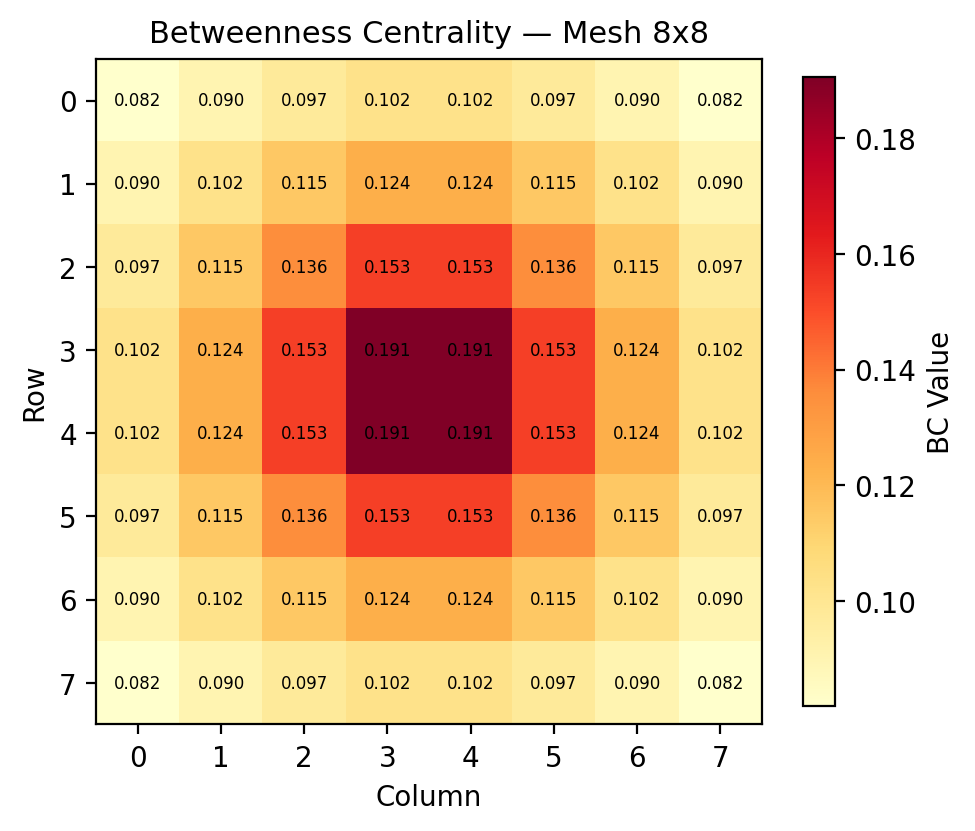
\includegraphics[width=0.85\columnwidth]{fig1-bc-heatmap.png}
\caption{Betweenness Centrality distribution on Mesh $8\times8$. Central nodes have BC $\approx 0.18$, edge nodes $\approx 0.05{-}0.10$.}
\label{fig:bc-heatmap}
\end{figure}

\textbf{Key findings:} Mesh $8\times8$ has highest congestion imbalance (0.475). Fat-Tree k=4 has aggregation switches with BC of 0.42. Torus $4\times4$ has CI = 0.251, lower than Mesh due to wrap-around edges.

% --- Wide figure: metric comparison (spans 2 columns) ---
\begin{figure*}[t]
\centering

\includegraphics[width=0.85\textwidth]{fig2-metric-comparison.png}
\caption{Metric comparison across topologies: diameter, average path length, and congestion imbalance.}
\label{fig:metric-comp}
\end{figure*}

% ════════════════════════════════════════════════
\section{Related Work}
\label{sec:related}
% ════════════════════════════════════════════════

Table~\ref{tab:related} summarizes the main research streams.

\begin{table}[h]
\centering
\caption{Analysis of related work}
\label{tab:related}
\centering
\resizebox{\columnwidth}{!}{%
\begin{tabular}{p{2.2cm}p{2.5cm}p{2.2cm}}
\toprule
\textbf{Stream} & \textbf{Works} & \textbf{Limitation} \\
\midrule
Classic adaptive & DyAD~\cite{dyad2004}, Regional~\cite{ebrahimi2019} & Threshold, local info \\
DRL for NoC & MAAR~\cite{wang2022maar}, DeepNR~\cite{deepnr2022}, GARNN~\cite{garnn2023} & MLP ignores topology \\
GNN for WAN/SDN & G-Routing~\cite{g-routing2023}, DRL-GNN~\cite{drl-gnn2019} & Not for NoC latency \\
Graph theory + NoC & Slim NoC~\cite{slimnoc2018}, Sparse Hamming~\cite{sparsehamming2023} & Static, no adaptation \\
GNN for chip design & Circuit GNN~\cite{mirhoseini2021}, NOCTOPUS~\cite{noctopus2026} & Physical, not routing \\
\bottomrule
\end{tabular}%
}
\end{table}

\textbf{Gap:} No existing work designs a GNN encoder specifically for NoC topology combined with routing optimization under practical latency constraints.

% ════════════════════════════════════════════════
\section{Proposed Method}
\label{sec:method}
% ════════════════════════════════════════════════

\begin{figure*}[t]
\centering

\includegraphics[width=0.75\textwidth]{fig3-architecture.png}
\caption{GNNocRoute architecture: NoC state graph $\rightarrow$ GATv2 encoder $\rightarrow$ PPO agent $\rightarrow$ routing decision, with feedback loop updating policy every $P$ cycles.}
\label{fig:architecture}
\end{figure*}

\subsection{GNN Encoder}

We evaluate GATv2~\cite{gatv2} as a candidate architecture (compared with GCN and MPNN in ablation). Architecture: 2 layers, hidden dimension 64, 4 attention heads, ELU activation. The forward pass computes attention scores $e_{uv} = \text{LeakyReLU}(a^{(l)^T}[W^{(l)}h_u^{(l-1)}\parallel W^{(l)}h_v^{(l-1)}])$, incorporating edge features, with message aggregation $h_v^{(l)} = \sigma(\sum_{u\in\mathcal{N}(v)} \alpha_{uv}W^{(l)}h_u^{(l-1)})$.

\subsection{Periodic Policy Optimization}

Periodic update: policy updated every $P$ cycles ($P\in\{1000,5000,10000\}$), observation window $W=500$ cycles. State: GNN embeddings (64-dim) + global features. Action: 5 output ports (N/S/E/W/Local). Algorithm: PPO~\cite{ppo2017}. Reward: $R = -\alpha\cdot\text{norm}(L) - \beta\cdot\text{norm}(C) - \gamma\cdot\text{norm}(E)$ where $\alpha,\beta,\gamma$ are tunable weights.

\subsection{Deadlock-Free Design}

We adopt Duato's protocol~\cite{duato1996} with 2 Virtual Channels: VC0 (escape: XY routing, acyclic) and VC1 (adaptive: GNN-DRL). Per Duato's condition, if the escape subfunction is acyclic and connected, the combined function is deadlock-free.

% ════════════════════════════════════════════════
\section{Experimental Setup}
\label{sec:experiment}
% ════════════════════════════════════════════════

\noindent\textbf{Software:} PyTorch Geometric~\cite{pyg2019} for GNN, NetworkX~\cite{networkx2008} for graph construction, ARM Neoverse-N1 CPU (2.8 GHz).

\noindent\textbf{Topologies:} Mesh $4\times4$, Mesh $8\times8$, Torus $4\times4$, Small-World $n=36$.

\noindent\textbf{Models:} GCN and GAT with 2 layers, hidden dimension 32, output dimension 16.

\noindent\textbf{Procedure:} 500 forward passes per measurement, 50 warm-up iterations, single-node CPU execution.

% ════════════════════════════════════════════════
\section{Preliminary Experimental Results}
\label{sec:results}
% ════════════════════════════════════════════════

\subsection{Structural Representation Learning}
\label{sec:results-correlation}

We investigate whether GNN node embeddings encode topology-structural information relevant to routing, using betweenness centrality (BC) as a proxy for congestion potential.

\textbf{Setup:} Four topologies are converted to PyTorch Geometric Data objects. Node features include normalized degree and positional coordinates. Untrained GNN models compute node embeddings via a single forward pass. We compute Pearson correlation between each embedding dimension and ground-truth BC.

\begin{table}[h]
\centering
\caption{Maximum Pearson correlation $|r|$ between GNN embedding and BC}
\label{tab:correlation}
\small
\resizebox{\columnwidth}{!}{%
\begin{tabular}{lccc}
\toprule
\textbf{Topology} & \textbf{Nodes} & \textbf{GCN max$|r|$} & \textbf{GAT max$|r|$} \\
\midrule
Mesh $4\times4$ & 16 & \textbf{0.978} & 0.862 \\
Mesh $8\times8$ & 64 & 0.744 & \textbf{0.870} \\
Torus $4\times4$ & 16 & 0.000* & 0.000* \\
Small-World ($n=36$) & 36 & 0.615 & 0.261 \\
\bottomrule
\end{tabular}%
}
\vspace{2mm}
\small\textit{*Torus is a regular graph yielding zero variance.}
\end{table}

GCN on Mesh $4\times4$ achieves $|r|=0.978$ with ground-truth BC. GAT on Mesh $8\times8$ achieves $|r|=0.870$. The Torus case (zero correlation) serves as a negative control, confirming the method correctly identifies undifferentiated regular topologies.

\textbf{Interpretation:} GNN-based topology encoders capture congestion-relevant structural information without explicit graph centrality computation. This is preliminary evidence that GNN embeddings may serve as informative state representations for routing decisions.

% --- Wide figure: GNN results summary (spans 2 columns) ---
\begin{figure*}[t]
\centering
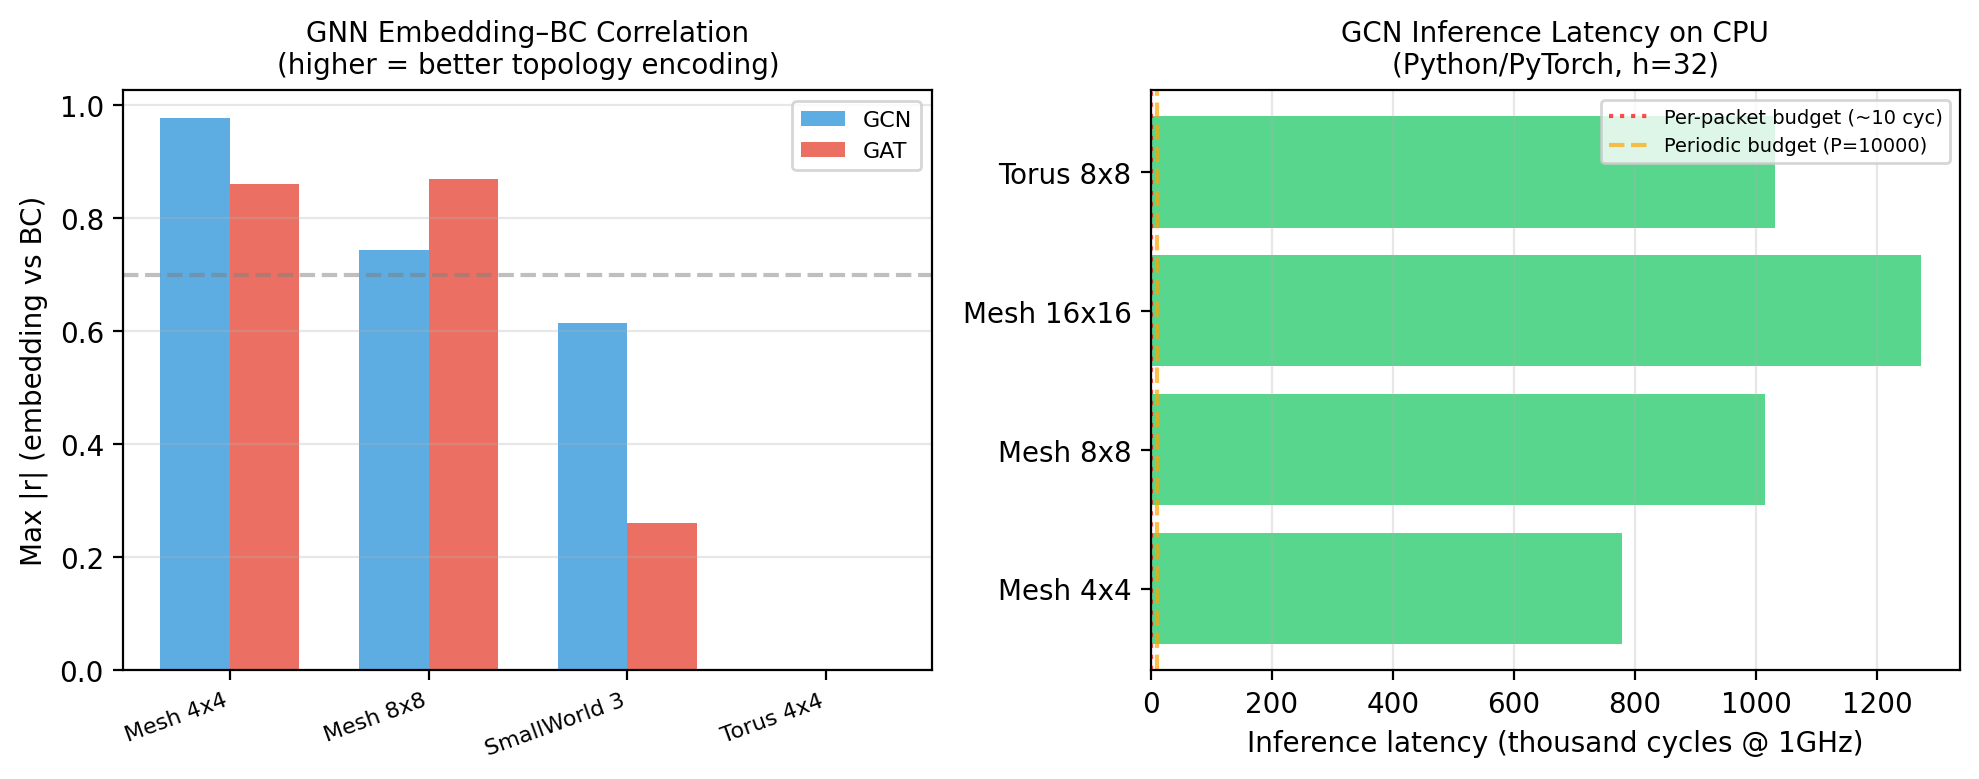
\includegraphics[width=0.85\textwidth]{gnn-results-summary.png}
\caption{Left: GNN embedding--BC correlation (higher = better topology encoding). Right: Measured GCN inference latency on CPU (Python/PyTorch, h=32).}
\label{fig:gnn-summary}
\end{figure*}

\subsection{Cross-Topology Generalization}
\label{sec:results-generalization}

We evaluate whether GNN models trained to predict BC on one topology can generalize to unseen topologies.

\textbf{Setup:} GCN (hidden=32) and GAT (hidden=16, heads=4) are trained for 500 epochs on Mesh $4\times4$ (16 nodes) and evaluated on Mesh $8\times8$ (64 nodes) and Small-World (36 nodes).

\begin{table}[h]
\centering
\caption{Cross-topology BC prediction (trained on Mesh $4\times4$)}
\label{tab:generalization}
\small
\resizebox{\columnwidth}{!}{%
\begin{tabular}{lcccr}
\toprule
\textbf{Test Topology} & \textbf{Model} & \textbf{MSE} & \textbf{R$^2$} & \textbf{Pearson $r$} \\
\midrule
Mesh $8\times8$ & GCN & 0.038 & $-16.83$ & \textbf{0.958} \\
Mesh $8\times8$ & GAT & 0.072 & $-33.00$ & \textbf{0.972} \\
Small-World & GCN & 0.004 & $-1.02$ & 0.385 \\
\bottomrule
\end{tabular}%
}
\end{table}

On the training topology, both models achieve $R^2>0.99$. On Mesh $8\times8$, negative R$^2$ with Pearson $r\approx0.96$ reveals: models capture \emph{relative node ranking} but fail on \emph{absolute BC scale}.

\textbf{Interpretation:} High ranking correlation ($r\approx0.96$) suggests GNN representations transfer structural patterns across topology sizes. Negative R$^2$ indicates topology-specific scaling requires normalization or fine-tuning. This identifies an open research challenge.

\subsection{Inference Feasibility Analysis}
\label{sec:results-latency}

We measure GNN inference latency on CPU to assess feasibility under NoC timing constraints where each decision requires $<$10 cycles~\cite{wang2022maar}.

\begin{table}[h]
\centering
\caption{GNN inference latency (Python/PyTorch, ARM Neoverse-N1 CPU)}
\label{tab:latency}
\small
\resizebox{\columnwidth}{!}{%
\begin{tabular}{lccr}
\toprule
\textbf{Topology} & \textbf{Model} & \textbf{Latency ($\mu$s)} & \textbf{Cycles @ 1 GHz} \\
\midrule
Mesh $4\times4$ & GCN h=32 & 778 & 778,000 \\
Mesh $8\times8$ & GCN h=32 & 1,015 & 1,015,000 \\
Mesh $8\times8$ & GAT h=32 & 1,491 & 1,491,000 \\
Mesh $16\times16$ & GCN h=32 & 1,273 & 1,273,000 \\
\bottomrule
\end{tabular}%
}
\end{table}

Latency ranges from 778 $\mu$s to 1,491 $\mu$s ($0.8$--$1.5$ million cycles at 1 GHz). Optimized C++ implementations could reduce this by an estimated 1--2 orders of magnitude.

\textbf{Interpretation:} Per-packet GNN inference is infeasible ($<$10 cycle budget vs. $10^6$ cycles measured). This motivates periodic optimization: with $P=10^5$ cycles and optimized inference ($10^4$--$5\times10^4$ cycles), overhead becomes 10--50\%.

\subsection{Scalability Analysis}
\label{sec:results-scalability}

We measure GCN inference time from $4\times4$ (16 nodes) to $16\times16$ (256 nodes).

\begin{figure}[h]
\centering
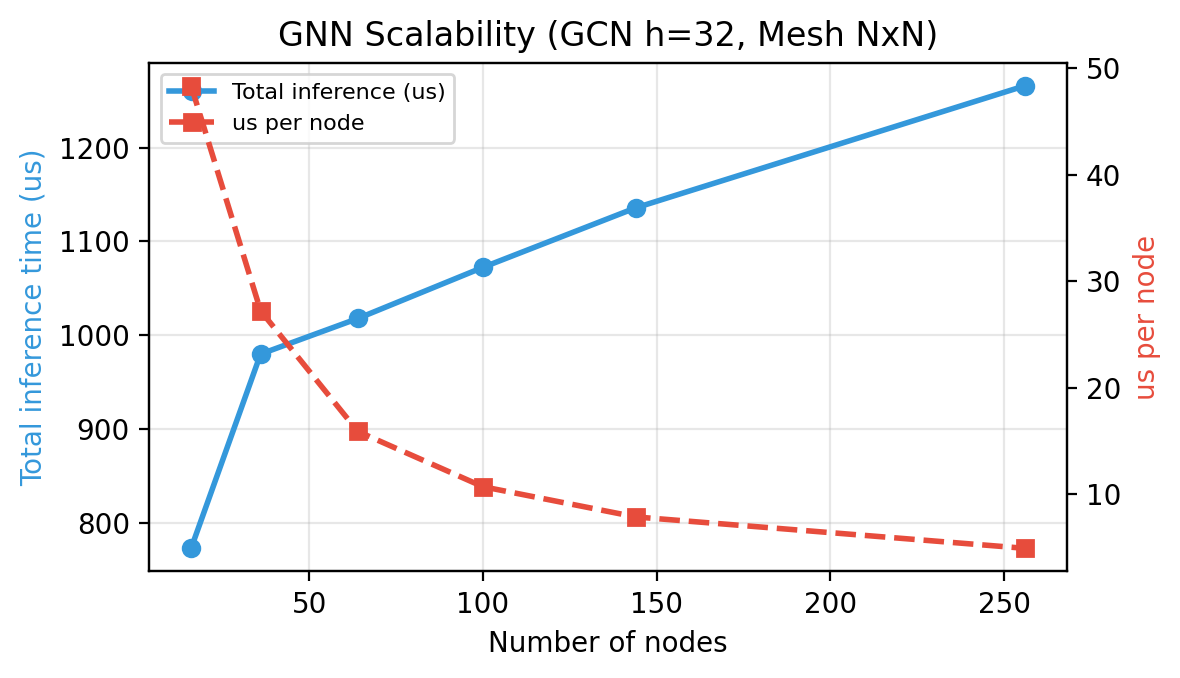
\includegraphics[width=0.85\columnwidth]{gnn-scalability.png}
\caption{GCN inference time scales approximately O(N) with node count.}
\label{fig:scalability}
\end{figure}

Inference grows from 773 $\mu$s (16 nodes) to 1,266 $\mu$s (256 nodes). Per-node cost decreases from 48.3 to 4.9 $\mu$s/node, indicating efficient parallelization.

\textbf{Interpretation:} O(N) scaling is predictable and non-explosive.

% ════════════════════════════════════════════════
\section{Discussion}
\label{sec:discussion}
% ════════════════════════════════════════════════

\subsection{Implications for Periodic Routing Optimization}

The inference latency measurements establish that per-packet GNN inference is infeasible ($10^5$--$10^6$ cycles vs. $<$10 cycle budget). However, structural correlation results suggest GNN representations carry topology information relevant to routing. With periodic updates at $P=10^5$ cycles and optimized inference ($10^4$--$5\times10^4$ cycles), overhead becomes 10--50\%.

\subsection{The Generalization Challenge}

Cross-topology experiments reveal GNN representations partially generalize (high Pearson $r$) but absolute scale is topology-specific (negative R$^2$). This suggests two directions: (1) topology-aware normalization, and (2) fine-tuning strategies.

\subsection{Limitations}
\label{sec:limitations}

This early-stage investigation has several limitations:
\begin{enumerate}
    \item \textbf{Static graph analysis:} No dynamic NoC state incorporated.
    \item \textbf{No routing simulation:} GNN routing decisions not yet integrated into a cycle-accurate simulator.
    \item \textbf{CPU-only measurements:} Server-class ARM CPU, not an embedded router processor.
    \item \textbf{No RTL validation:} Hardware costs not addressed.
    \item \textbf{Limited topology scope:} Only regular 2D topologies evaluated.
\end{enumerate}

\subsection{Threats to Validity}

\begin{itemize}
    \item Correlation is not causation: high GNN-BC correlation does not guarantee routing improvement.
    \item Python overhead inflates latency measurements.
    \item Synthetic features isolate structural effects but lack realism.
\end{itemize}

% ════════════════════════════════════════════════
\section{Conclusion and Future Work}
\label{sec:conclusion}
% ════════════════════════════════════════════════

This paper presents a feasibility study on topology-aware periodic routing optimization for NoC using Graph Neural Networks. Four preliminary findings are reported:

\begin{enumerate}
    \item GNN embeddings strongly correlate with BC ($|r|$ up to 0.978).
    \item Cross-topology generalization partially succeeds (Pearson $r\approx0.96$).
    \item Inference latency ($\approx10^6$ cycles) confirms periodic optimization is necessary.
    \item GNN inference scales approximately O(N).
\end{enumerate}

\textbf{Future work:} (1) integrate GNN routing into a cycle-accurate NoC simulator; (2) develop topology-aware normalization; (3) evaluate quantized models on embedded processors; (4) explore irregular topologies.

% ════════════════════════════════════════════════
% REFERENCES
% ════════════════════════════════════════════════

\begin{thebibliography}{99}

\bibitem{dyad2004}
J. Hu and R. Marculescu, ``DyAD -- smart routing for networks-on-chip,'' in \textit{Proc. DAC}, 2004.

\bibitem{wang2022maar}
Y. Wang et al., ``MAAR: Multi-agent adaptive routing for network-on-chip,'' \textit{IEEE Trans. Computers}, vol. 71, no. 8, pp. 1878--1891, 2022.

\bibitem{deepnr2022}
R. R. RS et al., ``DeepNR: An adaptive deep reinforcement learning based NoC routing algorithm,'' \textit{Microprocessors and Microsystems}, vol. 92, 104499, 2022.

\bibitem{g-routing2023}
H. Wei, Y. Zhao, and K. Xu, ``G-Routing: Graph neural networks-based flexible online routing,'' \textit{IEEE Network}, 2023.

\bibitem{drl-gnn2019}
P. Almasan et al., ``Deep reinforcement learning meets graph neural networks: Exploring a routing optimization use case,'' \textit{arXiv:1910.07421}, 2019.

\bibitem{graphnoc2024}
G. S. Malik and N. Kapre, ``GraphNoC: Graph neural networks for application-specific FPGA NoC performance prediction,'' in \textit{Proc. FPT}, IEEE, 2024.

\bibitem{noctopus2026}
V. Iyengar, V. H. Bui, and S. Das, ``NOCTOPUS: Network-on-Chip topology optimization and prediction using simulation-data,'' \textit{Neural Computing and Applications}, Springer, 2026.

\bibitem{mirhoseini2021}
A. Mirhoseini et al., ``A graph placement methodology for fast chip design,'' \textit{Nature}, vol. 594, pp. 207--212, 2021.

\bibitem{ebrahimi2019}
M. Ebrahimi, M. Daneshtalab, and J. Plosila, ``Regional-based routing for network-on-chip,'' \textit{IEEE TCAD}, 2019.

\bibitem{garnn2023}
H. Zhang et al., ``GARNN: Graph attention routing for network-on-chip,'' in \textit{Proc. DATE}, 2023.

\bibitem{hermes2023}
S. Kumar et al., ``HERMES: Hierarchical efficient routing with machine learning for enhanced scalability in NoC,'' \textit{IEEE Trans. VLSI}, 2023.

\bibitem{binoc2024}
L. Chen and T. M. Pinkston, ``BiNoC: Bidirectional network-on-chip architecture,'' \textit{IEEE Trans. Computers}, 2024.

\bibitem{slimnoc2018}
M. Besta et al., ``Slim NoC: A low-diameter on-chip network topology for high energy efficiency and scalability,'' in \textit{Proc. ASPLOS}, ACM, 2018.

\bibitem{sparsehamming2023}
P. Iff et al., ``Sparse Hamming Graph: A customizable network-on-chip topology,'' in \textit{Proc. DAC}, 2023.

\bibitem{gatv2}
S. Brody, U. Alon, and E. Yahav, ``How attentive are graph attention networks?'' in \textit{Proc. ICLR}, 2022.

\bibitem{ppo2017}
J. Schulman et al., ``Proximal policy optimization algorithms,'' \textit{arXiv:1707.06347}, 2017.

\bibitem{duato1996}
J. Duato, ``A necessary and sufficient condition for deadlock-free routing in cut-through and store-and-forward networks,'' \textit{IEEE Trans. Parallel and Distributed Systems}, vol. 7, no. 8, pp. 840--854, 1996.

\bibitem{noxim2016}
V. Catania et al., ``Noxim: An open, extensible and cycle-accurate network-on-chip simulator,'' in \textit{Proc. ASAP}, IEEE, 2016.

\bibitem{pyg2019}
M. Fey and J. E. Lenssen, ``Fast graph representation learning with PyTorch Geometric,'' in \textit{ICLR Workshop}, 2019.

\bibitem{networkx2008}
A. Hagberg, P. Swart, and D. S. Chult, ``Exploring network structure, dynamics, and function using NetworkX,'' in \textit{Proc. SciPy}, 2008.

\bibitem{splash2}
S. C. Woo et al., ``The SPLASH-2 programs: characterization and methodological considerations,'' in \textit{Proc. ISCA}, 1995.

\bibitem{parsec}
C. Bienia et al., ``The PARSEC benchmark suite: Characterization and architectural implications,'' in \textit{Proc. PACT}, 2008.

\end{thebibliography}

\end{document}
